\documentclass[a4paper, 14pt]{extarticle}
\usepackage[russian]{babel}
\usepackage[T1]{fontenc}
\usepackage{fontspec}
\usepackage{indentfirst}
\usepackage{enumitem}
\usepackage{graphicx}
\usepackage[
  left=20mm,
  right=10mm,
  top=20mm,
  bottom=20mm
]{geometry}
\usepackage{parskip}
\usepackage{titlesec}
\usepackage{xurl}
\usepackage{hyperref}
\usepackage{float}
\usepackage[
  figurename=Рисунок,
  labelsep=endash,
]{caption}
\usepackage[outputdir=build, newfloat]{minted}

\hypersetup{
  colorlinks=true,
  linkcolor=black,
  filecolor=blue,
  urlcolor=blue,
}

\renewcommand*{\labelitemi}{---}
\setmainfont{Times New Roman}
\setmonofont{JetBrains Mono}[
  SizeFeatures={Size=11},
]

\newenvironment{code}{\captionsetup{type=listing}}{}
\SetupFloatingEnvironment{listing}{name=Листинг}

\setminted{
  fontsize=\footnotesize,
  frame=lines,
  framesep=2mm,
}

\setlength{\parskip}{6pt}

\setlength{\parindent}{1cm}
\setlist[itemize]{itemsep=0em,topsep=0em,parsep=0em,partopsep=0em,leftmargin=2.0cm,wide}
\setlist[enumerate]{itemsep=0em,topsep=0em,parsep=0em,partopsep=0em,leftmargin=2.0cm,wide}

\renewcommand{\thesection}{\arabic{section}.}
\renewcommand{\thesubsection}{\thesection\arabic{subsection}.}
\renewcommand{\thesubsubsection}{\thesubsection\arabic{subsubsection}.}

\titleformat{\section}{\normalfont\bfseries}{\thesection}{0.5em}{}
\titleformat{\subsection}{\normalfont\bfseries}{\thesubsection}{0.5em}{}

\titleformat*{\section}{\normalfont\bfseries}
\titleformat*{\subsection}{\normalfont\bfseries}

\linespread{1.5}
\renewcommand{\baselinestretch}{1.5}

\begin{document}

\begin{titlepage}
  \vspace{0pt plus2fill}
  \noindent

  \vspace{0pt plus6fill}
  \begin{center}
    Санкт-Петербургский национальный исследовательский университет
    информационных технологий, механики и оптики

    \vspace{0pt plus3fill}

    Факультет инфокоммуникационных технологий

    Направление подготовки 11.03.02

    \vspace{0pt plus2fill}

    Лабораторная работа №3

    Разработка заданий с использованием Gulp

  \end{center}

  \vspace{0pt plus9fill}
  \begin{flushright}
    Выполнил: \\
    Швалов Даниил Андреевич

    Группа: К33211

    Проверила: \\
    Марченко Елена Вадимовна
  \end{flushright}

  \vspace{0pt plus2fill}
  \begin{center}
    Санкт-Петербург

    2023
  \end{center}
\end{titlepage}

\section{Введение}

\textbf{Цель работы}: научиться работать с утилитой автоматизации задач Gulp,
инструментом для отладки и тестирования BrowserSync, разработать форму для
отправки обратной связи с помощью PHP, локально развернуть WordPress.

\section{Ход работы}

\subsection*{Задание №1}

В данном задании необходимо настроить gulp следующий образом:
\begin{itemize}
  \item создать два таска – настроить на последовательное и параллельное
  выполнение;
  \item настроить отображение файлов проекта в браузере и автоматическую
  перезагрузку при изменении одного из контролируемых файлов проекта.
\end{itemize}

Для выполнения задания был инициализирован проект с помощью команды \texttt{npm
  init}. После выполнения данной команды в корне проекта появился файл
\texttt{package.json}, содержащий информацию о проекте (см. листинг
\ref{code:package.json}). Данный файл содержит название, версию и описание
зависимостей проекта.

\begin{code}
  \inputminted{json}{../task-1/package.json}
  \caption{Исходный код package.json}
  \label{code:package.json}
\end{code}

После этого в проект был установлен Gulp с помощью команды \texttt{npm i gulp}.
Также с помощью команды \texttt{npm i browser-sync} был установлен BrowserSync —
утилита, которая автоматически перезагружает измененные файлы и страницы,
синхронизирует навигацию между браузерами, а также позволяет тестировать сайт
сразу на нескольких устройствах.

В листинге \ref{code:gulp-series} представлен исходный код, создающий две
задачи, которые с помощью функции \texttt{gulp.series} запускаются
последовательно. На рис. \ref{fig:gulp-series} изображен результат выполнения
команды \texttt{gulp}.

\begin{code}
  \begin{minted}{js}
    const gulp = require("gulp");

    gulp.task("task-1", function (callback) {
        console.log("Task 1");
        callback();
    });

    gulp.task("task-2", function (callback) {
        console.log("Task 2");
        callback();
    });

    gulp.task("default", gulp.series("task-1", "task-2"));
  \end{minted}
  \caption{Исходный код Gulp за последовательного запуска задач}
  \label{code:gulp-series}
\end{code}

\begin{figure}[H]
  \centering
  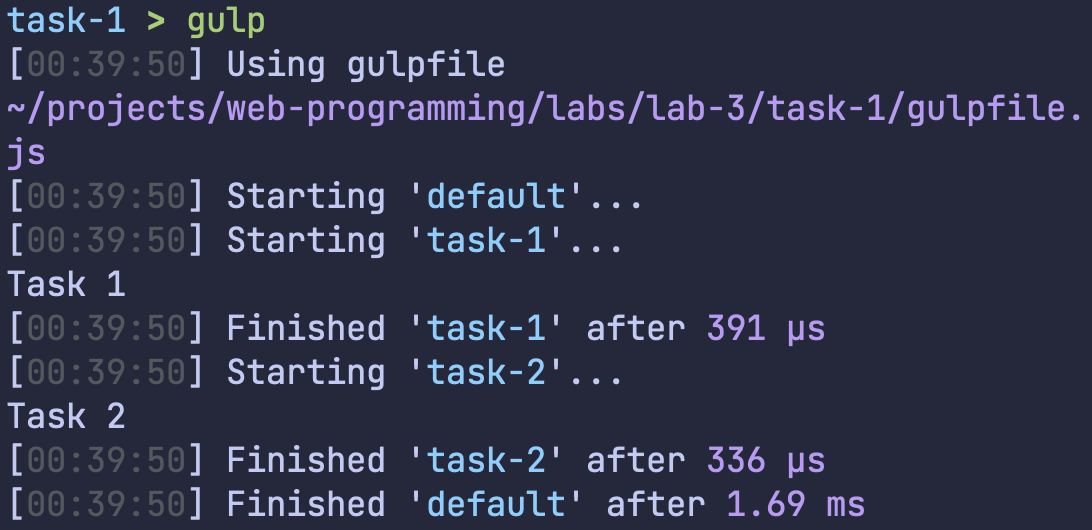
\includegraphics[width=0.8\textwidth]{images/gulp-series.png}
  \caption{Результат выполнения команды Gulp}
  \label{fig:gulp-series}
\end{figure}

В листинге \ref{code:gulp-parallel} представлен исходный код, который запускает
те же две задачи паралелльно с помощью функции \texttt{gulp.parallel}. На рис.
\ref{fig:gulp-parallel} изображен результат выполнения команды \texttt{gulp}.

\begin{code}
  \begin{minted}{js}
    const gulp = require("gulp");

    gulp.task("task-1", function (callback) {
        console.log("Task 1");
        callback();
    });

    gulp.task("task-2", function (callback) {
        console.log("Task 2");
        callback();
    });

    gulp.task("default", gulp.parallel("task-1", "task-2"));
  \end{minted}
  \caption{Исходный код Gulp за параллельного запуска задач}
  \label{code:gulp-parallel}
\end{code}

\begin{figure}[H]
  \centering
  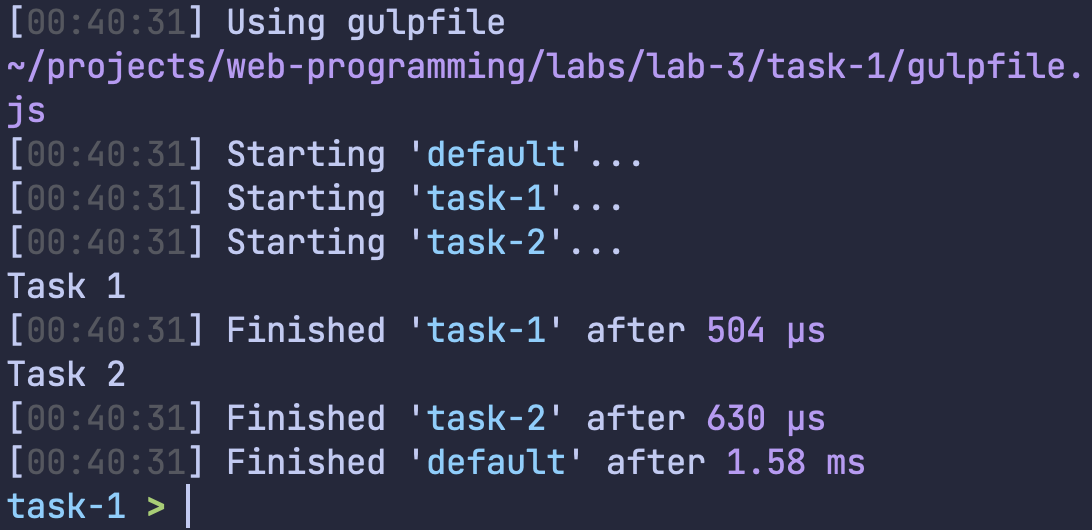
\includegraphics[width=0.8\textwidth]{images/gulp-parallel.png}
  \caption{Результат выполнения команды Gulp}
  \label{fig:gulp-parallel}
\end{figure}

В листинге \ref{code:gulp-browser-sync} представлен исходный код, который
создает задачу \texttt{browserSync}. Данная задача отслеживает изменения в
HTML-файлах, и при изменении перезагружает страницу веб-браузера. При выполнении
этой команды запустится сервер, который и будет отслеживать изменения файлов
(рис. \ref{fig:gulp-browser-sync} и \ref{fig:browser-before}).

\begin{code}
  \begin{minted}{js}
    const gulp = require("gulp");
    const browserSync = require("browser-sync").create();

    gulp.task("browserSync", function () {
        browserSync.init({
            server: {
            baseDir: "./",
            },
        });

        gulp.watch("*.html").on("change", browserSync.reload);
    });

    gulp.task("default", gulp.series("browserSync"));
  \end{minted}
  \caption{Исходный код Gulp за параллельного запуска задач}
  \label{code:gulp-browser-sync}
\end{code}

\begin{figure}[H]
  \centering
  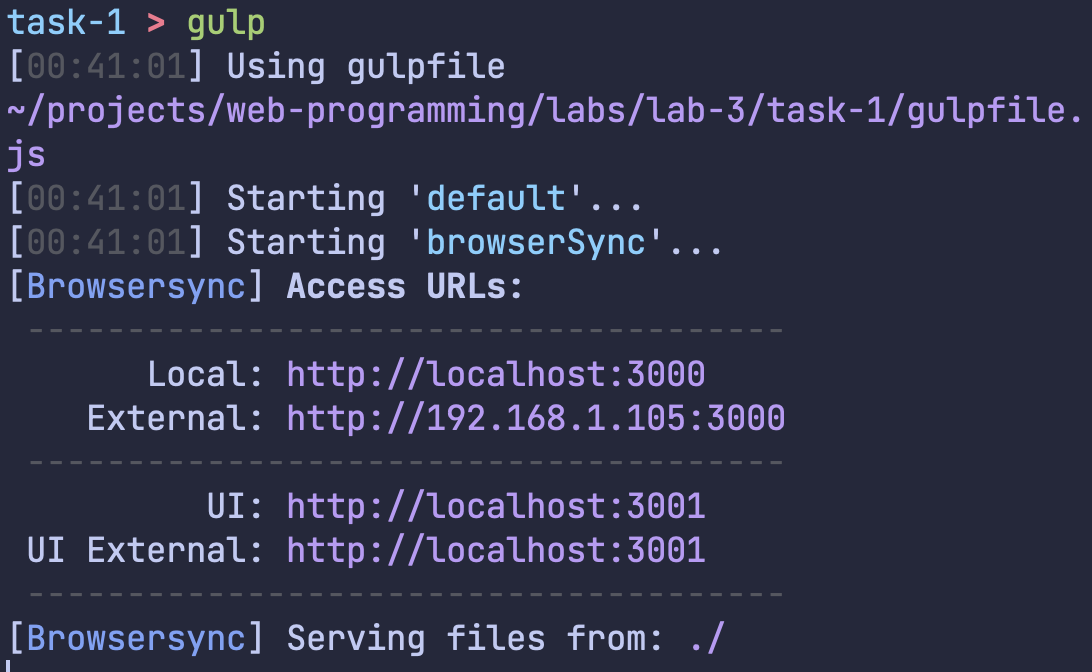
\includegraphics[width=0.8\textwidth]{images/gulp-browser-sync.png}
  \caption{Результат выполнения команды Gulp}
  \label{fig:gulp-browser-sync}
\end{figure}

\begin{figure}[H]
  \centering
  \fbox{
\includegraphics[width=0.9\textwidth]{images/browser-before.png}}
  \caption{Страница браузера до изменения}
  \label{fig:browser-before}
\end{figure}

При изменении содержимого \texttt{index.html} браузер автоматически
перезагрузится с новым содержимым (рис. \ref{fig:browser-after}).

\begin{figure}[H]
  \centering
  \fbox{
\includegraphics[width=0.9\textwidth]{images/browser-after.png}}
  \caption{Страница браузера после изменения}
  \label{fig:browser-after}
\end{figure}

\subsection*{Задание №2}

В данном задании необходимо создать форму для отправки информации по обратной
связи от пользователя сайта. В ней пользователь должен передать информацию о
себе: имя, фамилию, электронную почту, обратную связь. Также в форме должны быть
радио-кнопки (по меньшей мере 2 шт.) и должны быть чек-боксы (не менее трех).

Для хранения обратной связи в качестве СУБД была выбрана MySQL, поскольку это
очень популярная технология, на которую можно запросто найти множество полезной
информации по любому вопросу. Кроме того, в языке PHP есть встроенная
библиотека, позволяющая напрямую работать с MySQL, что сильно упрощает процесс
разработки.

В соответствии с заданием была сверстана форма, которая содержит следующие поля:
\begin{itemize}
  \item имя пользователя;
  \item фамилия пользователя;
  \item электронная почта пользователя;
  \item оценка качества обслуживания (от 1 до 5 в виде радио-кнопок);
  \item возможность отметить то, что понравилось больше всего (например,
  скорость обслуживания, простой и понятный интерфейс или широкий ассортимент
  товаров);
  \item комментарий, в котором пользователь может более подробно раскрыть свою
  обратную связь.
\end{itemize}

На рис. \ref{fig:feedback-clear-form} показана форма, получившаяся в итоге. При
ее заполнении (рис. \ref{fig:feedback-filled-form}) пользователь обязательно
должен указать свое имя, фамилию, электронную почту, а также поставить оценку
качества обслуживания. В дополнение, пользователь может отметить то, что ему
понравилось больше всего, а также написать комментарий, если это потребуется.
После того, как пользователь отправит обратную связь, его перекинет на страницу
с благодарностью (рис. \ref{fig:feedback-success}). На ней пользователя встретит
ссылка, которая позволит вернуться обратно на страницу заполнения формы обратной
связи, в случае, если он захочет оставить еще больше обратной связи.

\begin{figure}[H]
  \centering
  \fbox{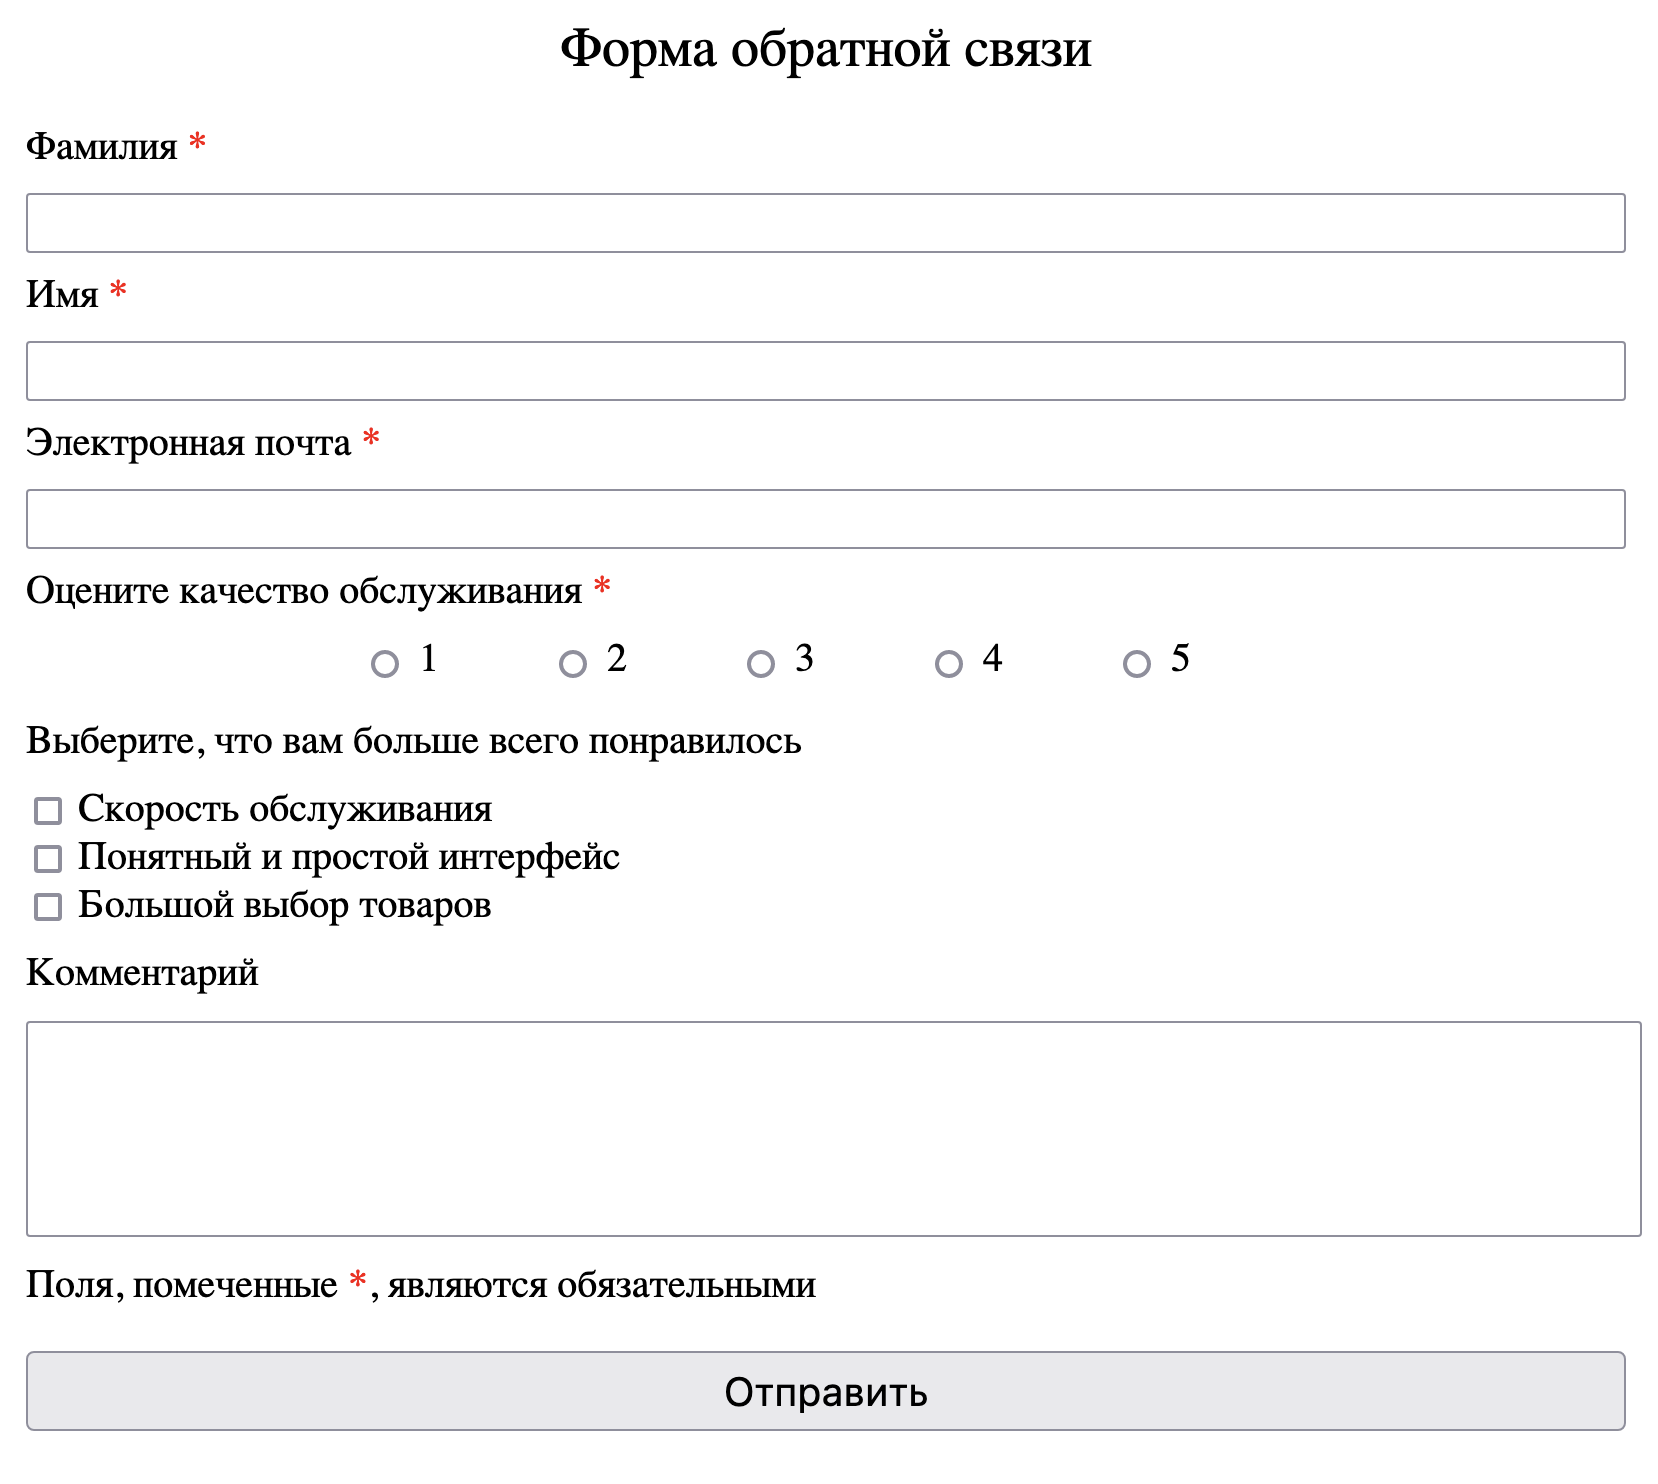
\includegraphics[width=0.8\textwidth]{images/feedback-clear-form.png}}
  \caption{Форма обратной связи}
  \label{fig:feedback-clear-form}
\end{figure}

\begin{figure}[H]
  \centering
  \fbox{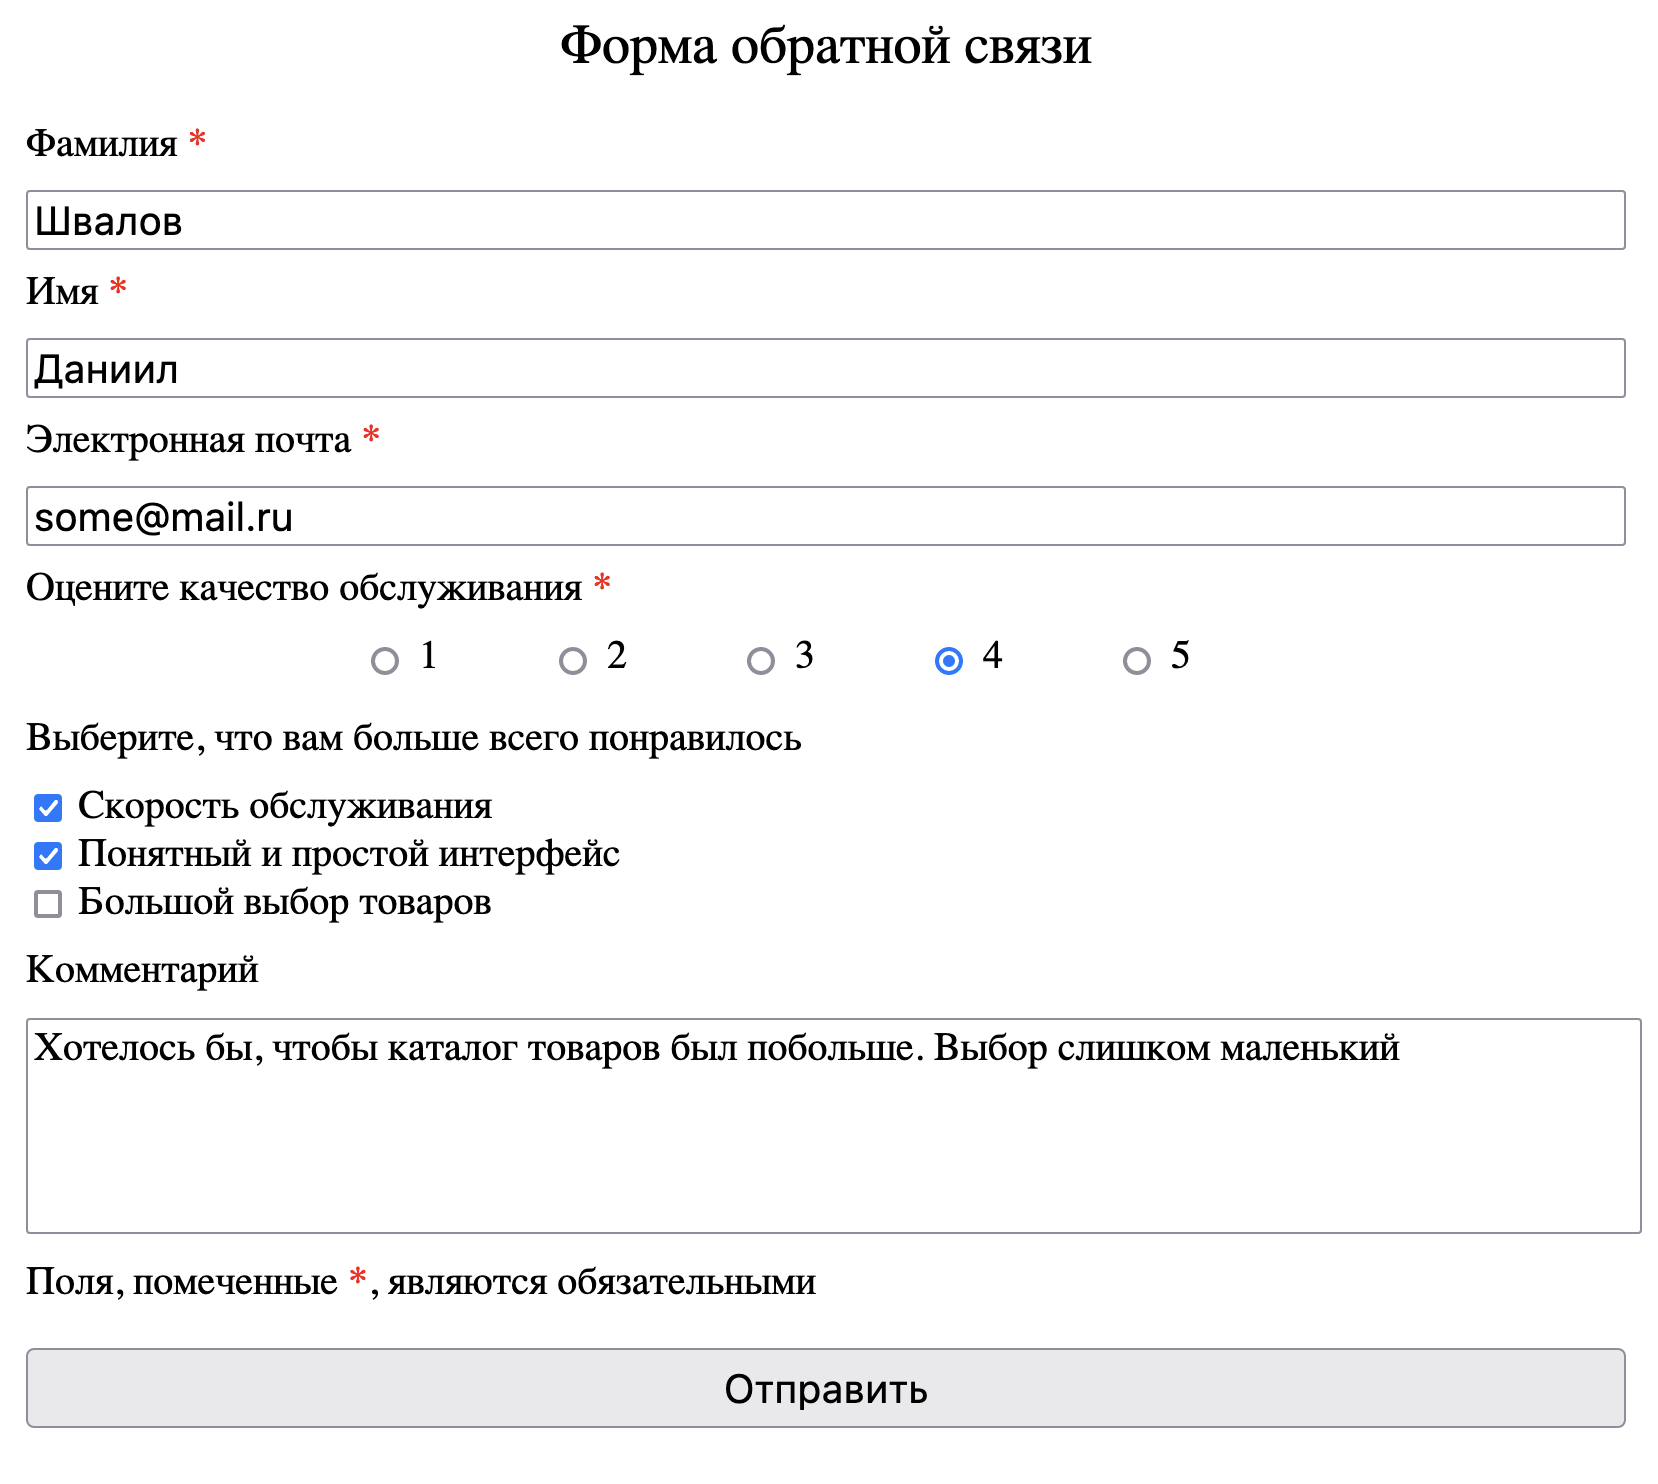
\includegraphics[width=0.8\textwidth]{images/feedback-filled-form.png}}
  \caption{Заполненная форма обратной связи}
  \label{fig:feedback-filled-form}
\end{figure}

\begin{figure}[H]
  \centering
  \fbox{
\includegraphics[width=0.9\textwidth]{images/feedback-success.png}}
  \caption{Страница после заполнения формы обратной связи}
  \label{fig:feedback-success}
\end{figure}

В приложениях \ref{app:index.html} и \ref{app:feedback-success.html} находится
исходный код HTML-страниц, изображенных на рис. \ref{fig:feedback-clear-form} и
\ref{fig:feedback-success} соответственно. В качестве обработчика POST-запроса
при отправке формы используется PHP-скрипт, исходный код которого расположен в
приложении \ref{app:feedback.php}. Код, использующийся для взаимодействия с
базой данных, был вынесен в отдельный файл, исходный код которого находится в
приложении \ref{app:database.php}. На рис. \ref{fig:database} изображена схема
получившейся базы данных.

\begin{figure}[H]
  \centering
  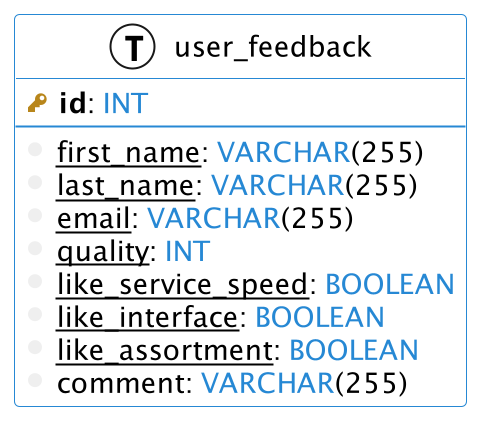
\includegraphics[width=0.4\textwidth]{images/puml/database.png}
  \caption{Схема базы данных}
  \label{fig:database}
\end{figure}

\subsection*{Задание №3}

В данном задании необходимо установить инструментарий для отладки проектов, а
также движок WordPress. После этого необходимо настроить сервер так, чтобы при
запросе по адресу \url{http://test.site} открывался портал WordPress.

В качестве веб-сервера, который будет отдавать статические файлы, такие как
HTML, CSS, PHP-скрипты, был выбран Nginx. Веб-сервер Nginx является достаточно
популярным решением в наше время, в сети Интернет находится большое количество
документации и примеров для Nginx, что позволяет быстро и просто найти решение
для той или иной проблемы. Также Nginx является высокоэффективным и
производительным решением, что подтверждается использованием этой технологии
множеством крупных компаний, занимающихся разработкой и настройкой
высоконагруженных систем.

В качестве СУБД была выбрана MySQL, поскольку это очень популярная технология,
на которую также можно запросто найти множество полезной информации по любому
вопросу. Кроме того, в языке PHP есть встроенная библиотека, позволяющая
напрямую работать с MySQL, что сильно упрощает процесс разработки. В добавок ко
всему, движок WordPress также очень хорошо интегрирован с MySQL.

Для развертывания собственного веб-сервера необходимо установить все выше
перечисленные инструменты. Nginx и MySQL были установлены с помощью пакетного
менеджера. WordPress был загружен с официального сайта.

После загрузки всех необходимых инструментов был настроен Nginx. Файл
конфигурации Nginx находится в приложении \ref{app:nginx.conf}. В конфигурации
настраивается HTTP-сервер, который прослушивает все входящие соединения на порту
8080. В качестве корневой директории, в которой находятся скрипты и статические
файлы, была указана директория WordPress. Также было настроено использования
PHP-скриптов в качестве главной страницы веб-сервера. После настройки Nginx был
запущен и сайт стал доступен по адресу \url{127.0.0.1:8080} (рис.
\ref{fig:wordpress-before-hosts}).

\begin{figure}[H]
  \centering
  \fbox{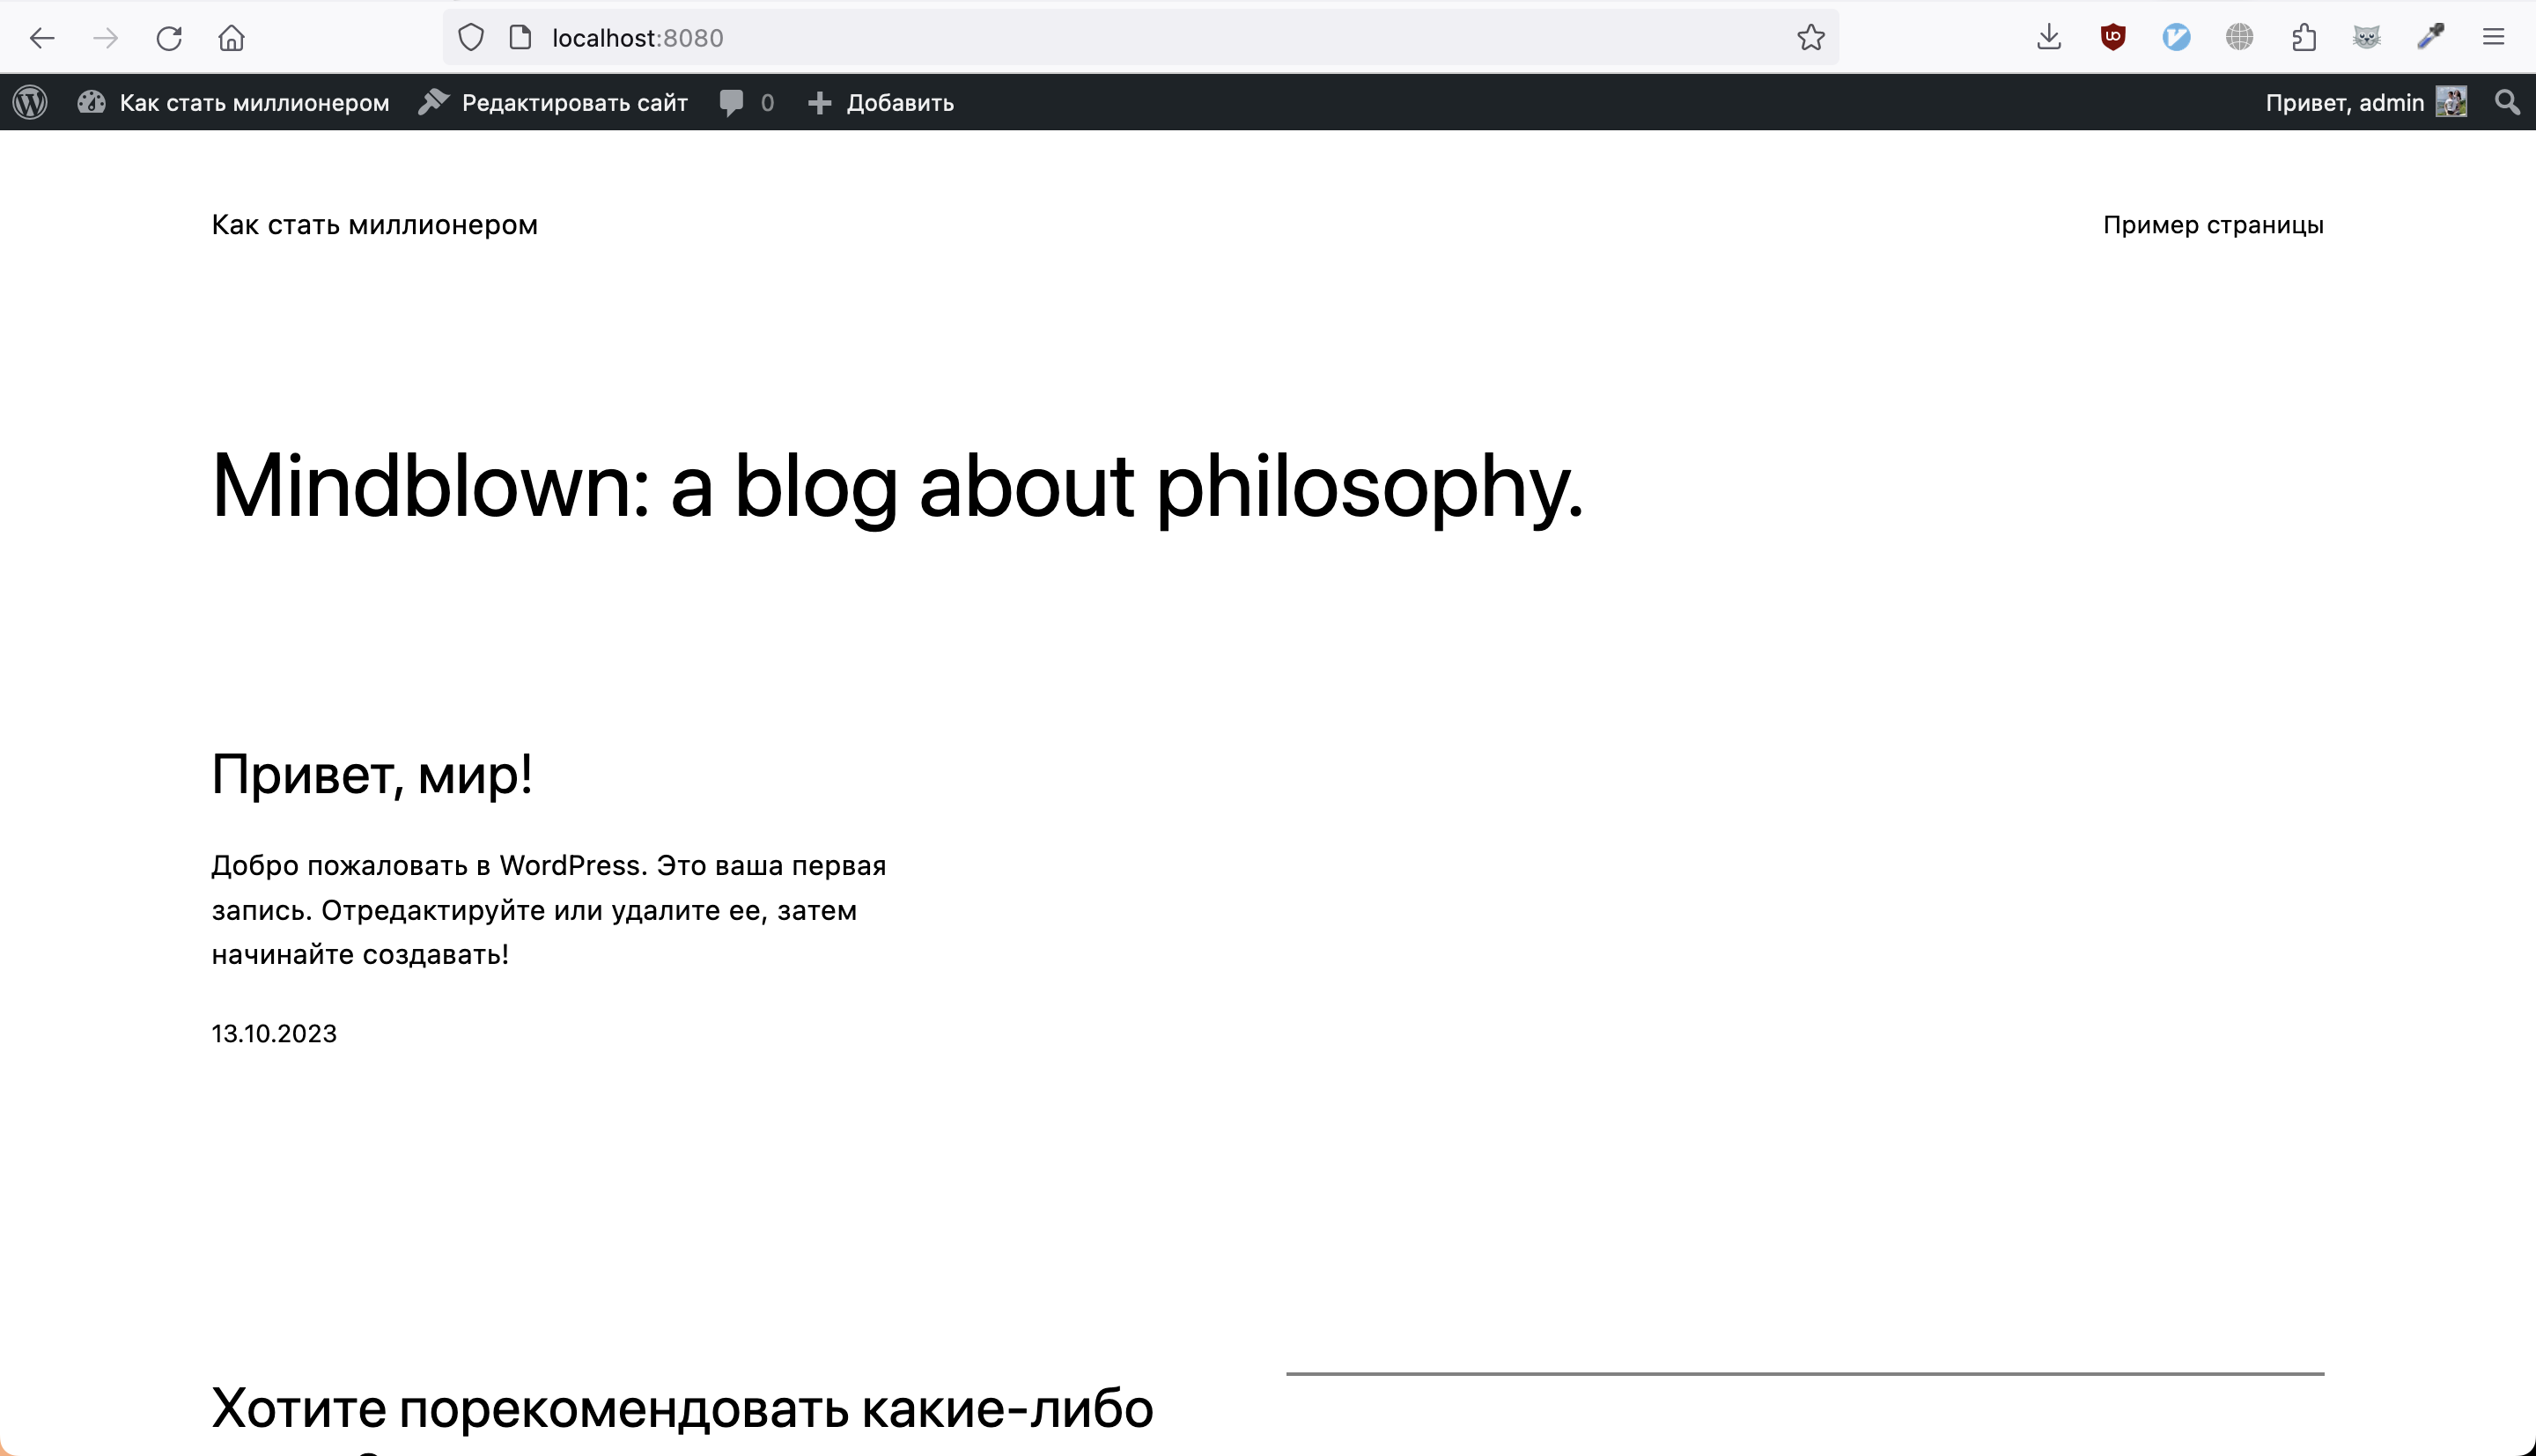
\includegraphics[width=0.9\textwidth]{images/wordpress-before-hosts.png}}
  \caption{Внешний вид сайта}
  \label{fig:wordpress-before-hosts}
\end{figure}

Для того, чтобы сайт был локально доступен по адресу \url{http://test.site},
необходимо в файл \texttt{/etc/hosts} добавить следующую строку:
\begin{minted}[frame=none]{text}
  127.0.0.1	test.site
\end{minted}
Файл hosts --- текстовый документ, который содержит в себе информацию о домене и
IP-адресе, который ему соответствует. Данная строка назначает домену test.site
IP-адрес 127.0.0.1, то есть адрес localhost.

После добавления необходимого адреса в файл \texttt{/etc/hosts}, портал
WordPress стал доступен по адресу \url{http://test.site} (рис.
\ref{fig:wordpress-after-hosts}).

\begin{figure}[H]
  \centering
  \fbox{
\includegraphics[width=0.9\textwidth]{images/wordpress-after-hosts.png}}
  \caption{Внешний вид сайта}
  \label{fig:wordpress-after-hosts}
\end{figure}

\section{Заключение}

\textbf{Вывод}: в данной лабораторной работе я научился работать с утилитой
автоматизации задач Gulp, инструментом для отладки и тестирования BrowserSync,
разработал форму для отправки обратной связи с помощью PHP, локально развернул
WordPress.

\newpage

\appendix

\titleformat{\section}[display]
{\normalfont\bfseries}
{\centering Приложение\ \thesection}
{0pt}{\centering}
\renewcommand{\thesection}{\Asbuk{section}}

\section{Исходный код страницы формы обратной связи}
\label{app:index.html}

\begin{code}
  \inputminted{html}{../task-2/index.html}
\end{code}

\newpage

\section{Исходный код страницы благодарности за заполнения формы обратной связи}
\label{app:feedback-success.html}

\begin{code}
  \inputminted{html}{../task-2/feedback-success.html}
\end{code}

\newpage

\section{Исходный код PHP-скрипта, обрабатывающего форму обратной связи}
\label{app:feedback.php}

\begin{code}
  \inputminted{php}{../task-2/feedback.php}
\end{code}

\newpage

\section{Исходный код PHP-скрипта, взаимодействующий с базой данных}
\label{app:database.php}

\begin{code}
  \inputminted{php}{../task-2/database.php}
\end{code}

\newpage

\section{Исходный код конфигурации Nginx}
\label{app:nginx.conf}

\begin{code}
  \inputminted{text}{../task-3/nginx.conf}
\end{code}

\end{document}
